\begin{figure}[H]
    \begin{subfigure}[t]{.5\textwidth}
        \caption{}
        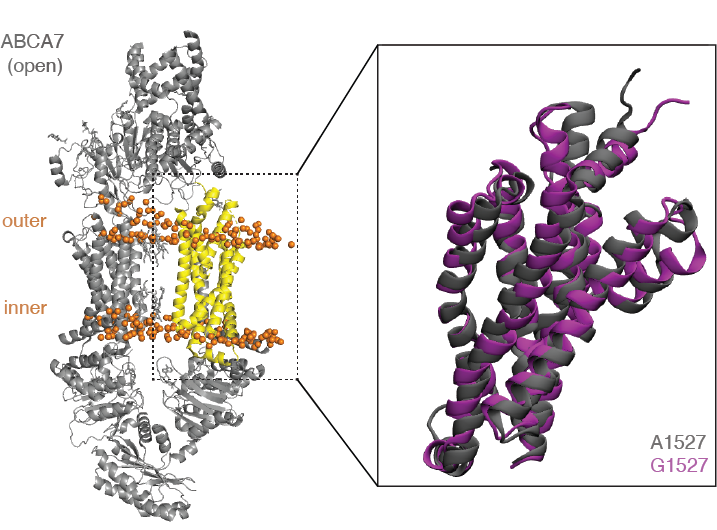
\includegraphics[width=\textwidth]{./extended_plots/abca7_structure_with_inset.png}        
    \end{subfigure}
    \hspace{1cm}
    \begin{subfigure}[t]{.3\textwidth}
        \caption{}
        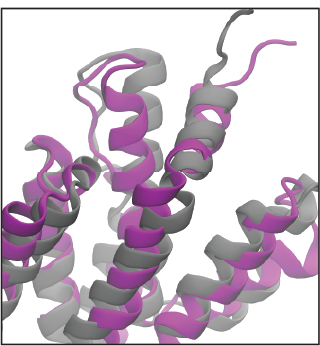
\includegraphics[width=\textwidth]{./extended_plots/abca7_structure_inset_only.png}        
    \end{subfigure}
    \par
    \begin{subfigure}[t]{.5\textwidth}
        \caption{}
        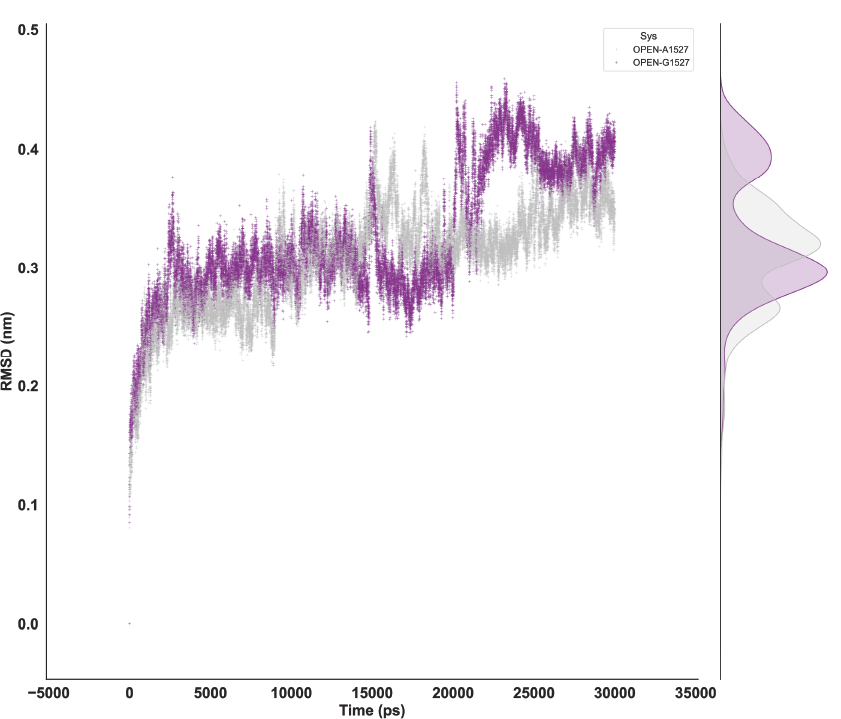
\includegraphics[width=\textwidth]{./extended_plots/rmsd_time.png}        
    \end{subfigure}
    \hspace{1cm}
    \begin{subfigure}[t]{.3\textwidth}
        \caption{}
        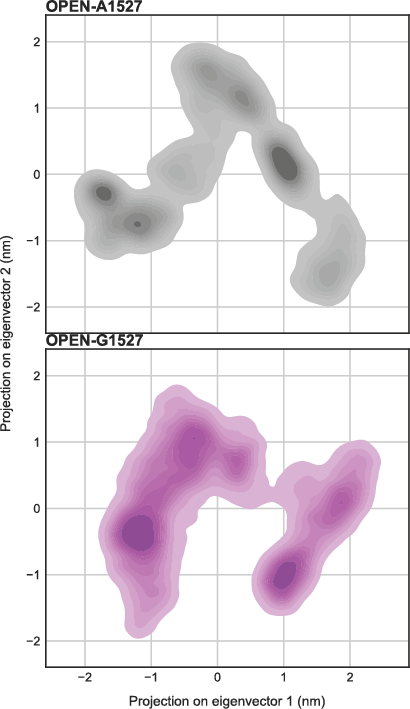
\includegraphics[width=\textwidth]{./extended_plots/rmsd_projection_open.png}        
    \end{subfigure}
    \par
    \begin{subfigure}[t]{.5\textwidth}
        \caption{}
        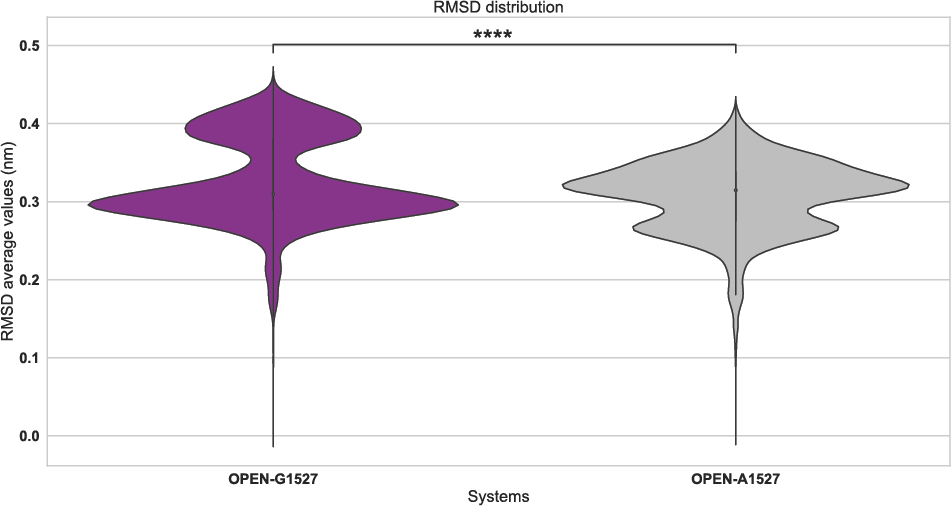
\includegraphics[width=\textwidth]{./extended_plots/rmsd_volcano.png}        
    \end{subfigure}
    \caption{
        \textbf{Molecular Dynamics Simulations of ABCA7 open conformations with p.Ala1527Gly substitution.}\\
    }
    \label{fig:md_simulations}
\end{figure}
\begin{itemize}
    \item[\textbf{(A)}] Open conformation ABCA7 protein structure. ABCA7 domain between residues 1517 and 1756 used for simulations is shown in yellow. Expanded yellow domain (inset from left), with A1527 variant (light grey) and G1527 variant (purple). 
    \item[\textbf{(B)}] Expanded inset from A with residues of interest rendered. 
    \item[\textbf{(C)}] Root mean squared deviations of open conformation domains from B with A1527 (light grey) or G1527 (purple) under simulation. Structural deviations over time were computed with respect to reference open structures from B. 
    \item[\textbf{(D)}] Projection of $C_\alpha$ atom positional fluctuations under simulation onto the first two principal components, for open conformation domain from B with A1527 (top, light grey) or G1527 (bottom, purple). 
    \item[\textbf{(E)}] Violin plot indicating average $C_\alpha$ atom positional fluctuations over time. 
\end{itemize}